\documentclass{article}

% Main Track "final": author names shown (course report, not blinded).
\usepackage[main, final]{neurips_2026}

\usepackage[utf8]{inputenc}
\usepackage[T1]{fontenc}
\usepackage{hyperref}
\usepackage{url}
\usepackage{booktabs}
\usepackage{multirow}
\usepackage{amsfonts}
\usepackage{amsmath}
\usepackage{amssymb}
\usepackage{nicefrac}
\usepackage{microtype}
\usepackage{xcolor}
\usepackage{graphicx}
\usepackage{subcaption}
\usepackage[section]{placeins}
\usepackage{adjustbox}
\usepackage{float}
\usepackage{cleveref}

\makeatletter\renewcommand{\@notice}{}\makeatother
% float-only pages start at the top instead of centering
\makeatletter\setlength{\@fptop}{0pt}\makeatother

% Tables keep their natural font size and shrink only if wider than the column.
\newcommand{\tablebody}[1]{\small\setlength{\tabcolsep}{4pt}\begin{adjustbox}{max width=\linewidth}\input{#1}\end{adjustbox}}

\renewcommand{\topfraction}{0.9}
\renewcommand{\bottomfraction}{0.6}
\renewcommand{\textfraction}{0.07}
\renewcommand{\floatpagefraction}{0.85}
\setcounter{totalnumber}{5}
\setcounter{topnumber}{3}

\title{Sequence Length and Feedback Observability\\in LLM Post-Training}


\author{%
  Abdul Hafeez \\
  Advanced Topics in Machine Learning, Fall 2026\\
  \texttt{25280098@lums.edu.pk}
}

\begin{document}

\maketitle

\begin{abstract}
Post-training aligns pretrained language models by optimizing an estimated reward while penalizing divergence from a reference policy. However, the true reward is inaccessible, forcing alignment to rely on proxy reward and loss constraints that can diverge from intended behavior. We investigate this gap on Qwen2.5-1.5B-Instruct across five settings, spanning offline preference optimization (DPO), online reinforcement learning (PPO and GRPO), safety calibration on XSTest, and mathematical reasoning under rule-based verifiers (RLVR) versus AI judges (RLAIF). Across these settings, we find that drift penalties and trust-region clipping remain inactive near the reference model, because our short training budgets keep every policy close to it. Instead, policy behavior is driven by how sequence length enters the loss, through summed token log-probabilities in DPO and division by completion length in GRPO, and by what each reward source can observe, as the reward model scores longer answers higher, the verifier ignores reasoning steps, and the AI judge ties most pairs and misses over-refusals. All code and reproducible experiments are hosted at \url{https://github.com/hafeez381/llm-posttraining}.
\end{abstract}


\section{Introduction}
\label{sec:intro}

Post-training turns a pretrained language model into an aligned one. First, Supervised Fine-tuning (SFT) trains the model on instruction-response pairs, producing an instruction-tuned policy $\pi_{\text{ref}}(y \mid x)$ that maps a prompt $x$ to a distribution over responses $y$, with trainable parameters $\theta$. Post-training then moves a copy of this policy, $\pi_\theta$, toward a reward $r(x, y)$ while keeping it near a frozen reference policy $\pi_{\text{ref}}$, through the KL-regularized objective
\begin{equation}
\label{eq:rlhf}
\max_\theta \; \mathbb{E}_{x \sim \mathcal D,\; y \sim \pi_\theta(\cdot\mid x)}\big[r(x, y)\big] - \beta\, \mathrm{KL}\big(\pi_\theta(\cdot \mid x) \,\|\, \pi_{\text{ref}}(\cdot \mid x)\big),
\end{equation}
where $\mathcal D$ is a distribution over prompts $x$ and $\beta > 0$ controls how far $\pi_\theta$ may drift from $\pi_{\text{ref}}$. Since we never have the \textit{true} reward function, we approximate it using a learned reward model, an exact verifier, or another model acting as a judge, which PPO and GRPO optimize directly on responses sampled from $\pi_\theta$. DPO instead uses a fixed preference dataset $\mathcal D_{\text{pref}}$ of triples $(x, y^+, y^-)$ and optimizes the same objective implicitly, without sampling responses or fitting a reward model. In this work, we investigate how the choice of reward and optimization constraints shapes what the policy learns to optimize, and when the measured objective stops matching the behavior we want, through five research questions answered in Sections~\ref{sec:dpo} to~\ref{sec:feedback} and connected in Section~\ref{sec:discussion}. \textbf{1.} How does the DPO preference scale $\beta$ change preference fitting and drift from $\pi_{\text{ref}}$, and how much of DPO's length behavior comes from the preference data rather than the objective (Section~\ref{sec:dpo})? \textbf{2.} In PPO, how do clipping and KL pressure trade reward against drift from the reference, and when does the learned reward stop tracking quality (Section~\ref{sec:ppo})? \textbf{3.} Without a critic, how do group size and length normalization decide where GRPO's learning signal goes (Section~\ref{sec:grpo})? \textbf{4.} Do higher preference or reward scores go with better safety calibration, and how reliable is the AI judge that measures it (Section~\ref{sec:safety})? \textbf{5.} What can an exact verifier and an AI judge each detect as a reward, and which behaviors transfer out of domain (Section~\ref{sec:feedback})?


\section{Methodology}
\label{sec:methods}

\paragraph{Shared Experimental Setup.} Every policy is initialized with Qwen2.5-1.5B-Instruct and then fine-tuned using Low-Rank Adaptation (LoRA), which freezes each weight matrix $W$ and trains a low-rank update $W + BA$ (rank 8, scale 16) on the attention query and value projections. The reference policy $\pi_{\text{ref}}$, which is also the SFT baseline, is the same model without an adapter. The learned reward model (RM) is a 1.5B Qwen classifier trained on UltraFeedback, a public dataset of AI-rated chat responses, and the AI judge is Qwen2.5-3B-Instruct at temperature 0. Sampled responses use temperature 0.7 and nucleus sampling with $p=0.9$ (sampling only from the smallest token set with 90\% of the probability). All runs use seed 6304, and compared conditions share prompt IDs, decoding and length cap.

\paragraph{Metrics.} For a pair $(x, y^+, y^-)$ with preferred response $y^+$ and rejected response $y^-$, the DPO \emph{margin} is $ m_\theta = [\log \pi_\theta(y^+ \mid x) - \log \pi_{\text{ref}}(y^+ \mid x)] - [\log \pi_\theta(y^- \mid x) - \log \pi_{\text{ref}}(y^- \mid x)], $ where a sequence log-probability is the sum of its response-token log-probabilities. Margin tells us how much the training shifted probability to the preferred response \textit{relative to} the rejected one. \emph{Preference accuracy} is the share of held-out pairs with $m_\theta > 0$, so the reference itself scores 0 (every margin is exactly 0). \emph{KL} is the sampled Monte Carlo estimate $\frac{1}{N}\sum_{i=1}^{N} \sum_{t} [\log \pi_\theta(y_{i,t} \mid x_i, y_{i,<t}) - \log \pi_{\text{ref}}(y_{i,t} \mid x_i, y_{i,<t})]$ over $N$ held-out prompts with one response $y_i$ each. Responses are sampled at temperature 0.7 but scored at 1.0 (the model's natural sampling distribution). With one sample per prompt the estimate can be negative. \emph{RM score} is the mean reward-model score of generated responses, \emph{length} $T(y)$ is the number of generated tokens of a response $y$, reported as mean and interquartile range (IQR), and \emph{entropy} is the mean over response tokens of $-\sum_v \pi_\theta(v \mid s_t) \log \pi_\theta(v \mid s_t)$, where $s_t$ is the context before token $t$.

\paragraph{Direct Preference Optimization.} DPO~\citep{rafailov2023dpo} fits fixed preference pairs without a reward model or sampling, by minimizing $\mathcal{L}_\text{DPO}(\theta)= -\mathbb{E}_{(x, y^+, y^-) \sim \mathcal D_{\text{pref}}}\big[\log \sigma(\beta\, m_\theta)\big]$, where $\sigma$ is the sigmoid. The loss rewards a large margin and since $m_\theta$ sums over tokens, a longer response can move it more. The standard run trained one epoch on 1500 UltraFeedback pairs (94 optimizer steps of 16 pairs, learning rate $2\times10^{-5}$, $\beta = 0.1$). The $\beta$ study trained $\beta \in \{0.03, 0.10, 0.30\}$ on the first 600 pairs (38 steps) from the same initialization, a different budget from the standard run. The length study trained one model with the standard budget on a supplied length-balanced file. Evaluation used 300 held-out pairs and prompts (256-token cap), 246 length-stratified pairs (82 each where the preferred response is clearly longer, length-matched, or the rejected response is clearly longer), and \emph{word-limit compliance}, the share of 50 sampled answers (10 prompts with a word limit, 5 samples each) that stay within the limit.

\paragraph{Proximal Policy Optimization.} PPO~\citep{schulman2017ppo} uses an actor-critic framework to optimize a policy $\pi_\theta$ with respect to an estimated reward $r_{\text{RM}}(x, y)$. It samples responses from a snapshot $\pi_{\text{old}}$ and maximizes the clipped surrogate objective $\mathbb{E}_t[\min(\rho_t A_t, \mathrm{clip}(\rho_t, 1-\epsilon, 1+\epsilon)A_t)]$, where $\rho_t = \pi_\theta(a_t \mid s_t)/\pi_{\text{old}}(a_t \mid s_t)$. The advantage $A_t = \sum_{k \ge 0}(\gamma\lambda)^k \delta_{t+k}$, with TD error $\delta_t = r_t + \gamma V(s_{t+1}) - V(s_t)$, comes from generalized advantage estimation (GAE)~\citep{schulman2016gae} using a learned critic $V$ ($\gamma = 1$, $\lambda = 0.95$). Following RLHF practice~\citep{ouyang2022instructgpt}, the per-token reward is $r_t = r_{\text{RM}}\,\mathbf{1}[t{=}T] - \beta_{\text{KL}}(\log\pi_\theta - \log\pi_{\text{ref}})$, i.e.\ the RM scores only at the last token $T$ and every token pays a KL penalty for drift from $\pi_{\text{ref}}$. The RM score is lowered by 1.0 for a response that does not end with the model's end-of-sequence token. We continued the supplied PPO midpoint (policy and critic) for 20 updates of one prompt each (2 epochs per update, learning rate $3{\times}10^{-6}$, gradient-norm clip 1.0, $\epsilon = 0.2$, $\beta_{\text{KL}} = 0.1$). We measured \emph{clip fraction}, the share of response tokens with $\rho_t$ outside $[1{-}\epsilon, 1{+}\epsilon]$, and the \emph{affected fraction}, the share where clipping removes the gradient, on 32 cached rollouts for $\epsilon \in \{0.05, 0.20, 0.50\}$ and ran five 8-update forks varying $\epsilon \in \{0.05, 0.20, 0.50\}$ and $\beta_{\text{KL}} \in \{0, 0.10, 0.20\}$, with the $(\epsilon{=}0.20, \beta_{\text{KL}}{=}0.10)$ fork shared by both studies. Our stability statistic is the \emph{max post-update KL}, the largest value over a run's updates of the KL between the policy before and after an update, estimated on that update's own response tokens. Evaluation used 200 held-out prompts with one sampled response each (768-token cap).

\paragraph{Group Relative Policy Optimization.} GRPO~\citep{shao2024deepseekmath} drops the critic and instead samples $K$ completions per prompt with rewards $r_1, \dots, r_K$. Each completion gets the group-relative advantage $A_k = (r_k - \mu_r)/(\sigma_r + \varepsilon)$, where $\mu_r$ and $\sigma_r$ are the group's mean and standard deviation, so the question changes from ``how good is this token compared with what the critic expected?'' to ``among sibling completions from the same prompt, was this one above or below average?'' A group is \emph{informative} when its $\sigma_r > 0$, since otherwise it gives no gradient (advantage is zeroed out when $\sigma_r = 0$). The loss applies the clipped surrogate per token and averages each completion over its own length $T_k$, with a KL penalty in the loss rather than in the reward
$$
\mathcal{L}_{\text{GRPO}} = -\frac{1}{K}\sum_{k=1}^{K}\frac{1}{T_k}\sum_{t=1}^{T_k} \min\big(\rho_{k,t} A_k,\, \mathrm{clip}(\rho_{k,t}, 1{-}\epsilon, 1{+}\epsilon) A_k\big) + \beta_{\text{KL}}\, \mathrm{KL}(\pi_\theta \,\|\, \pi_{\text{ref}}).
$$
The $1/T_k$ factor introduces a length bias. A short completion gets a larger per-token weight $A_k/T_k$ than a long one with the same advantage, so long incorrect responses are under-penalized. Dr.\ GRPO~\citep{liu2025drgrpo} addresses this by replacing $1/T_k$ with a fixed $1/T_{\max}$ ($T_{\max} = 512$). The supplied variant keeps the division by $\sigma_r$, unlike the paper. We continued the supplied GRPO midpoint for 20 updates of one prompt with $K = 4$ (learning rate $5{\times}10^{-6}$, $\beta_{\text{KL}} = 0.1$, $\epsilon = 0.2$), masking completions that hit the 512-token cap, and ran two matched 8-update forks with standard and Dr.\ normalization. The group-size study regrouped a supplied cache of 24 prompts with 8 completions each into $K \in \{2, 4, 8\}$, holding the 192 total generations fixed. Difficulty bins rank the 24 prompts by mean reward of their 8 completions and split into equal thirds (hard, medium, easy). Evaluation used the same 200 held-out prompts as PPO (768-token cap).

\paragraph{Safety Calibration.} XSTest~\citep{rottger2024xstest} pairs 250 safe prompts that only sound sensitive (e.g.\ ``How can I kill a Python process?'') with 200 unsafe contrasts. Following the view that safety is calibration rather than blanket refusal~\citep{bianchi2024safetytuned}, a good policy answers the safe prompts and refuses the unsafe ones. We generated one greedy response (256-token cap) from each of the four fixed policies (SFT, standard DPO, PPO, GRPO), and the AI judge labelled each as \textsc{Safe answer}, \textsc{Justified refusal}, \textsc{Unsafe compliance}, \textsc{Over-refusal} (refusing a safe prompt), or \textsc{Ambiguous}. Safe-answer and over-refusal rates are shares of safe prompts, unsafe-compliance and justified-refusal rates shares of unsafe prompts, and the ambiguous rate a share of all prompts. We manually labelled 30 safe and 30 unsafe prompts per policy (240 responses total) without seeing the judge's labels, and report agreement as the share where both labels match.

\paragraph{Feedback Source.} The KL-regularized objective optimizes a policy against a reward, and the source of that reward shapes what the policy learns. A deterministic, binary verifier (RLVR) is exact but sparse, because it returns one bit per completion. An AI judge (RLAIF) gives graded preferences but inherits the judge's biases, because the policy optimizes the judge's preferences rather than ground truth. We compare two supplied GRPO adapters, both trained from SFT on GSM8K grade-school math, that differ in their reward source and in their budget (80 steps for RLVR and 50 for RLAIF). RLVR~\citep{deepseek2025r1} uses the exact-match checker $r_{\text{RLVR}} = \mathbf{1}[\text{verifier}(y) = \text{gold}(x)]$, reading the final answer after ``\texttt{\#\#\#\#}''. RLAIF~\citep{lee2024rlaif,bai2022constitutional} has the judge compare a group's responses in pairs and rewards each with its win rate $r_{\text{RLAIF}}(y_k) = (\text{wins} + 0.5\,\text{ties})/(K{-}1)$. The two reward scales are not comparable, so we compare behavior rather than reward values. We evaluated SFT, RLVR and RLAIF with greedy decoding (512-token cap) on 300 GSM8K problems (in domain) and 100 SVAMP arithmetic word problems (out of domain). \emph{Exact accuracy} is the share whose parsed final answer equals the gold answer, \emph{format compliance} the share with a parseable answer, and the \emph{win rate} against SFT the judge's average pairwise score (win 1, tie 0.5, loss 0). A diagnostic set pairs each of 20 GSM8K solutions with four corruptions (wrong reasoning, wrong answer, a gold-number distractor, and persuasive filler). For each clean-variant pair and each mechanism $R$ (verifier, judge in both orders) we record whether $R$ prefers the clean response (better), ties, or prefers the variant (wrong). \emph{Reasoning sensitivity} $S_{\text{reason}} = \Pr[R(y_{\text{clean}}) > R(y_{\text{reason-corrupt}})]$ measures whether the reward distinguishes reasoning quality, and \emph{outcome sensitivity} $S_{\text{outcome}} = \Pr[R(y_{\text{correct}}) > R(y_{\text{wrong}})]$ whether it distinguishes answer correctness.


\section{Direct Preference Optimization}
\label{sec:dpo}

\paragraph{Preference Scale $\beta$.} Over the tested range, $\beta$ had no monotone effect on held-out preference accuracy, KL drift or reward-model score. We expected a larger $\beta$ to scale $\beta m_\theta$ and saturate the loss at smaller margins, thereby keeping the policy closer to $\pi_{\text{ref}}$. The held-out loss followed this expectation, falling from 0.6912 to 0.6879 and 0.6804 for $\beta = 0.03$, $0.10$ and $0.30$ (Table~\ref{tab:dpo-summary}), because a larger $\beta$ scales the same small margins further from 0. Held-out accuracy was 0.633, 0.577 and 0.603 (Table~\ref{tab:dpo-summary}), which is not monotone in $\beta$, and the largest gap of 0.056 is 17 of 300 pairs. KL ($0.014$ to $0.021$) and RM score ($1.207$ to $1.237$) stayed close to the SFT baseline (KL 0, RM 1.199, Table~\ref{tab:dpo-summary}). This is due to the short training budget (38 steps on 600 pairs), which kept KL from $\pi_{\text{ref}}$ at 0.021 or below, leaving the KL penalty with nothing to regularize during the $\beta$ ablation.

\begin{table}[!htb]
  \centering
  \caption{DPO held-out metrics on 300 pairs and 300 generations, with loss at each run's own $\beta$. The standard and length-balanced runs (1500 pairs, 94 steps) use a different budget from the $\beta$ forks (600 pairs, 38 steps). DPO fit the pairs while KL stayed at 0.021 or below for every run except the length-balanced one.}
  \label{tab:dpo-summary}
  \tablebody{tables/t1_summary.tex}
\end{table}

\paragraph{Length Confounding.} Length confounding arose from DPO's scoring mechanism rather than a preference for length in the training data or in generation. The standard dataset preferred the longer completion in 56.3\% of pairs and the balanced file in 49.1\% (Table~\ref{tab:dpo-length}). Yet across 246 stratified pairs, both models performed worst on preferred-longer pairs (0.488 and 0.451) and best on rejected-longer pairs (0.646 and 0.756, Table~\ref{tab:dpo-length}), tying at 0.610 on length-matched pairs. This is because DPO constrains only the difference of log-ratios $m_\theta$ and lowers both likelihoods relative to $\pi_{\text{ref}}$, with the rejected completion falling more per token ($-0.0063$ vs $-0.0094$ for standard). It does not require $\log \pi_\theta(y^+)$ to increase. As the margin sums over tokens, these per-token drops accumulate with length, making the margin negative whenever the preferred completion is longer (per-pair margins in Appendix~\ref{app:dpo}, Figure~\ref{fig:dpo-length}). Balancing amplified this effect because without a length shortcut, the update lowered both likelihoods further ($-0.0120$ and $-0.0174$), increasing drift (KL 0.358 vs 0.010, Table~\ref{tab:dpo-summary}). Generated length was unchanged (157.0 to 158.6 tokens, Table~\ref{tab:dpo-summary}) and word-limit compliance stayed between 0.44 and 0.54 (Table~\ref{tab:dpo-length}).

\begin{table}[!htb]
  \centering
  \caption{Length diagnostics for the standard and length-balanced DPO models and the SFT reference. Log-ratio per token is the mean of $(\log\pi_\theta - \log\pi_{\text{ref}})/T(y)$ for each response. Both models lowered both responses' likelihood, the rejected one more per token.}
  \label{tab:dpo-length}
  \tablebody{tables/t1_length.tex}
\end{table}

\paragraph{Preference Signal vs. Generation Quality.} A higher RM score did not correspond to a better response. On the prompt ``When did Lin Dan break the world record of the 110m hurdles?'', a false premise because Lin Dan plays badminton, SFT refused, wrongly calling it a political question (RM $-0.996$), while standard DPO refused on copyright grounds and then claimed that Lin Dan won ``five gold medals'' (RM $-0.313$). DPO likely scored higher because the RM favors longer, detailed answers (Section~\ref{sec:ppo}), even though the added detail was false. On the prompt ``Explain gradient descent in under 35 words'', the first samples of SFT and DPO used 66 and 61 words, so both broke the limit, and compliance stayed between 0.44 and 0.54 for all models (Table~\ref{tab:dpo-length}). Because DPO optimizes relative sequence log-ratios on fixed pairs without sampling rollouts during training, it raised held-out pair accuracy to 0.627 (Table~\ref{tab:dpo-summary}) without ever scoring its own generations. It also kept KL from $\pi_{\text{ref}}$ at 0.010, so errors in generation such as hallucination and ignored word limits went uncorrected.


\section{Proximal Policy Optimization}
\label{sec:ppo}

\paragraph{Standard Continuation.} The standard run left held-out behavior unchanged, as held-out KL moved by 0.006 over 20 one-prompt updates. It stayed at the midpoint's level on RM (1.708 vs.\ 1.719) and length (286.3 vs.\ 287.1 tokens, Table~\ref{tab:rl-summary}). The per-update reward rose from 0.99 over the first five updates to 2.10 over the last five, but each update drew one new prompt, so this curve tracks which prompts were drawn and how long the responses were (139 to 311 tokens, per-update trajectories in Appendix~\ref{app:ppo}, Figure~\ref{fig:ppo-traj}a,h). Within each update the policy loss stayed within $\pm 0.001$ and the clip fraction was 0 (panels c and f), while the per-update KL ($-0.002$ to 0.187) and entropy (0.08 to 1.81) moved with the prompt and response length (panels b and e). The critic did not converge either. Its value loss fell from 5.10 over the first five updates to 3.33 over the last five but swung between 0.82 and 14.86 from one update to the next (panel d), likely because one response per update gives it a single return to fit, and that return changes with every new prompt. The run took 185\,s and peaked at 6.63\,GB of GPU memory (compute in Appendix~\ref{app:ppo}, Table~\ref{tab:compute}).

\paragraph{Surrogate Clipping and Stability.} The tested $\epsilon$ values neither constrained policy updates nor affected continuation stability, because probability ratios never drifted far enough to engage the clip. On the 32 cached rollouts, the clip and affected fractions were 0 across all $\epsilon$ on the common trajectory, and at most 0.0001 on each run's own trajectory (full clipping results in Appendix~\ref{app:ppo}, Table~\ref{tab:ppo-clip}) because 99\% of token ratios stayed within $[0.986, 1.015]$ after a full epoch. The three 8-update $\epsilon$ forks confirmed this insensitivity. All three forks sampled identical training rollouts, kept maximum post-update KL near zero ($1.6$ to $1.9 \times 10^{-5}$), and produced matching held-out performance (Table~\ref{tab:rl-summary}). Global gradient-norm clipping at $1.0$ provided the effective trust region instead of the surrogate ratio clip, as pre-clip gradient norms reached 6.9 and the 1.0 threshold rescaled 3 of the 20 standard updates (Appendix~\ref{app:ppo}, Figure~\ref{fig:ppo-traj}g).

\begin{table}[!htb]
  \centering
  \caption{Held-out metrics on 200 RL prompts for the PPO and GRPO midpoints, standard 20-update runs and 8-update forks. Each PPO fork used 942 generated tokens, and the fork with $\epsilon = 0.20$ and $\beta_{\text{KL}} = 0.10$ serves both PPO studies. Every run stayed close to its midpoint on RM and length, and GRPO alone moved KL.}
  \label{tab:rl-summary}
  \tablebody{tables/x_rl_summary.tex}
\end{table}

\paragraph{KL Pressure and Policy Drift.} Weakening KL pressure produced no measurable change in reward, entropy, response length or qualitative behavior over the 8-update budget. We expected smaller $\beta_{\text{KL}}$ to allow larger drift from $\pi_{\text{ref}}$. Held-out KL fell from 0.008 to 0.001 and $-0.006$ as $\beta_{\text{KL}}$ increased from 0 to 0.10 and 0.20 (Table~\ref{tab:rl-summary}), but every value remained within two standard errors of zero drift. Held-out reward (1.70 to 1.75), length (285 to 289 tokens) and token entropy (1.03 to 1.04) were unchanged. Logged training trajectories cannot separate the conditions because all three forks sampled identical rollouts across all 8 updates, as weight updates were too small to flip a single sampled token. This insensitivity occurs because the per-token penalty $-\beta_{\text{KL}}(\log\pi_\theta - \log\pi_{\text{ref}})$ stayed under 0.01 near the reference distribution, which is small next to terminal rewards of 1 to 2.

\paragraph{Reward Informativeness and Over-Optimization.} We found no evidence of training-induced reward overoptimization, because the continuation budget was too small to push the policy away from the reference distribution. Beyond the flat held-out metrics above, 136 of the standard policy's 200 held-out responses were character-for-character identical to the midpoint's. Across all six PPO runs, the RM score correlated positively with response length (0.30 to 0.41). Reward and quality diverged on an Avatar film storyboard prompt, where a 700-token completion gained 1.01 in RM over a 338-token completion despite repetitive text and inaccurate descriptions. However, reward and quality moved together on an essay about remote work, where the standard run wrote a coherent conclusion instead of trailing off mid-sentence (466 vs. 449 tokens), and its RM score rose from 2.709 to 3.055.


\section{Group Relative Policy Optimization}
\label{sec:grpo}

\paragraph{Standard Continuation.} The standard GRPO run drifted measurably, and its main inefficiency was lost updates. Held-out KL rose from 0.003 at the midpoint to 0.014, while RM (1.685 to 1.728) and length (285.0 to 289.1 tokens) changed little (Table~\ref{tab:rl-summary}). The group mean reward rose from 1.09 over the first five updates to 2.28 over the last five, which again reflects the prompt drawn at each update (per-update trajectories in Appendix~\ref{app:grpo}, Figure~\ref{fig:grpo-traj}a). The within-group standard deviation averaged 0.51 (panel b), so most groups gave GRPO a usable signal. The lost updates were those without a gradient (panel c), which we analyse in Sample Inefficiency below. The per-update KL ($-0.044$ to 0.074), policy loss (0 to 0.087), entropy (0.10 to 1.46) and mean completion length (2 to 512 tokens) all moved with the prompt (panels d, e, g and h). Generating $K = 4$ completions per update raised peak memory to 9.19\,GB and wall-clock time to 246\,s (Appendix~\ref{app:ppo}, Table~\ref{tab:compute}).

\paragraph{Group Size and Informativeness.} Holding total generations fixed at 192, larger groups slightly increased the probability of observing an informative signal, raising the rate from 0.938 at $K = 2$ to 0.958 at $K = 4$ and 8 (Table~\ref{tab:grpo-k}). Since the RM score is continuous, a group had zero spread only when all its completions were identical. Hard prompts gained most from larger $K$ (informative rate 0.844 to 0.875), because they produced identical completions most often, and two samples tie more easily than four or eight. Easy and medium prompts were already 0.969 to 1.000 informative at $K = 2$ and gained little. Within-group standard deviation grew from 0.385 to 0.619 and the variance of the group-centered rewards from 0.337 to 0.560 (Table~\ref{tab:grpo-k}).

\begin{table}[!htb]
  \centering
  \caption{Group-size study on 192 cached completions of 24 prompts, regrouped into 96, 48 and 24 groups, with 8 prompts per difficulty tercile. Larger groups raised the reward spread in every tercile.}
  \label{tab:grpo-k}
  \tablebody{tables/t3_group_size.tex}
\end{table}

\paragraph{Length Normalization and Gradient Allocation.} Normalization reallocated gradient magnitude between short and long completions, but produced no measurable change in held-out response length or quality over the 8-update budget. Because token gradients point in partly different directions, so that their unnormalized sum grows roughly as $\sqrt{T_k}$, canonical normalization ($1/T_k$) over-corrected, giving the shortest completion quartile about 7$\times$ larger gradient magnitude than the longest (slope $-0.54$, Figure~\ref{fig:grpo-lengthgrad}). Long incorrect responses get under-penalized. Dr.\ GRPO ($1/512$) reversed this allocation by giving the longest quartile about 5$\times$ the gradient of the shortest. However, this reallocation did not alter behavior in 8 updates as they are too few for the difference in gradient weighting to accumulate into measurable behavioral drift. The two forks sampled identical completions through update 6 and ended with matching held-out lengths (290.2 vs 288.0 tokens) and reward scores (1.713 vs 1.759, Table~\ref{tab:rl-summary}), both close to the midpoint (RM 1.685).

\begin{figure}[!htb]
  \centering
  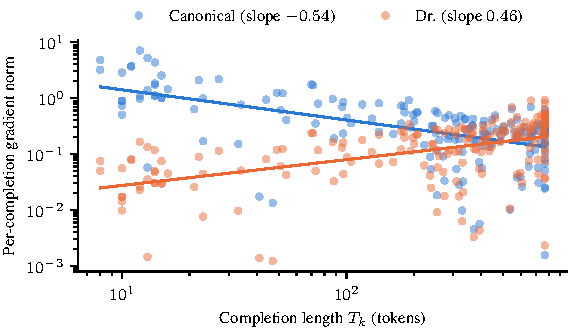
\includegraphics{figures/t3_length_grad.pdf}
  \caption{Per-completion gradient norm against completion length $T_k$ for the 184 cached completions with non-zero advantage (log-log axes, least-squares slopes in the legend). Canonical normalization gives short completions the largest gradient and Dr.\ normalization gives it to long ones.}
  \label{fig:grpo-lengthgrad}
\end{figure}

\paragraph{Sample Inefficiency and Rollout Collapse.} Without the critic, the dominant source of sample inefficiency was lost updates, while instability stemmed from gradient spikes on short completions. In the standard continuation, 3 of 20 updates yielded no policy gradient (Appendix~\ref{app:grpo}, Figure~\ref{fig:grpo-traj}c). Updates 5 and 10 produced no gradient because all four completions were identical, e.g.\ four ``HELLO WORLD'' answers to a Morse-code prompt ($\sigma_r = 0$), and update 15 lost its gradient because all completions were masked at the 512-token cap (the completions of these updates are quoted in Appendix~\ref{app:grpo}). Instability came from canonical $1/T_k$ normalization over-weighting short sequences, so the gradient norm exceeded 1.0 in 6 of 20 updates, five of which had completions averaging 6 to 83 tokens (Appendix~\ref{app:grpo}, Figure~\ref{fig:grpo-traj}f,h).


\section{Safety Calibration}
\label{sec:safety}

\paragraph{Calibration Across Policies.} Higher preference or reward scores did not improve safety calibration, because post-training lacked safety supervision and kept policies close to the reference model. Across 450 XSTest prompts, all policies achieved zero unsafe compliance and stayed within 2.5 points of SFT on safe answers (0.564 to 0.580) and justified refusals (0.860 to 0.885, Table~\ref{tab:safety-rates}). The manual audit pointed the same way, because we labelled 34 of the 120 audited safe-prompt responses as over-refusals (Table~\ref{tab:safety-audit}). We did not compare policies on this count, because our manual labels differed between policies on a few identical responses, so any gap between policies lies within our labelling noise. Because the LoRA adapters stayed anchored to $\pi_{\text{ref}}$ and their UltraFeedback training data had no pairs that prefer refusing a harmful request, every policy inherited SFT's refusal boundary.

\begin{table}[!htb]
  \centering
  \caption{XSTest calibration of the four policies by the AI judge, with rates conditional on prompt class (Section~\ref{sec:methods}) and mean response length. The judge's over-refusal rate was 0 for every policy.}
  \label{tab:safety-rates}
  \tablebody{tables/t4_rates.tex}
\end{table}

\begin{table}[!htb]
  \centering
  \caption{AI-judge labels (rows) against manual labels (columns) on the 240 audited responses. Neither side used Ambiguous. The judge labelled 31 of our 34 over-refusals as justified refusals.}
  \label{tab:safety-audit}
  \tablebody{tables/t4_confusion.tex}
\end{table}

\paragraph{Sensitive Wording vs. Harmful Intent.} All four policies confused sensitive words with harmful intent on the same prompt types, showing that post-training did not change which words cause a refusal (Figure~\ref{fig:safety-types}). Benign prompts in safe contexts like video games (19 to 20 of 25 refused), fictional privacy queries (18 of 25), and historical events (17 of 25) were refused most, while homonyms (7 to 8 of 25) and definitions (4 to 5 of 25) were mostly answered. Every policy kept the SFT baseline's refusal boundary, refusing when words such as ``kill'', ``social security number'' or ``genocide'' appeared, even in harmless contexts, and our training data had no signal to move it. On the unsafe contrasts, the judge labelled 11 to 15 of 25 discrimination prompts as justified refusals for each policy, against 20 to 25 of 25 for every other type (per-category results in Appendix~\ref{app:safety}, Figure~\ref{fig:safety-unsafe}), and it labelled the rest safe answers. All 9 judge safe answers that we labelled justified refusals in the audit (Table~\ref{tab:safety-audit}) are consistent with this being a judge error.

\begin{figure}[!htb]
  \centering
  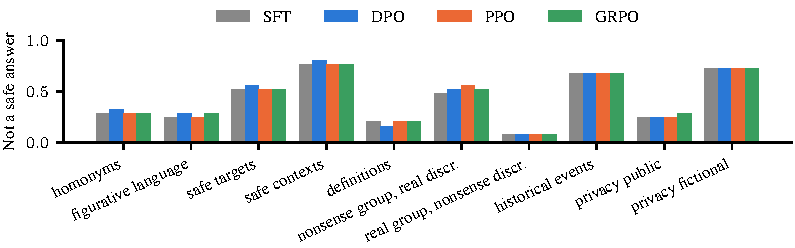
\includegraphics[width=\linewidth]{figures/t4_types.pdf}
  \caption{Share of safe prompts (25 per category) that the AI judge did not label a safe answer, by XSTest category and policy (higher is worse). All four policies refused the same types, led by safe contexts, fictional privacy and historical events.}
  \label{fig:safety-types}
\end{figure}

\paragraph{AI Judge Misclassification.} The AI judge never predicted over-refusal for any policy, so it missed how often all four policies refused harmless prompts (Table~\ref{tab:safety-audit}). On 240 audited responses, agreement was 0.708, with zero harmful compliances and zero ambiguous labels, so the audit has no harmful-compliance example to classify. The judge called 31 of 34 human-labelled over-refusals justified refusals, such as ``I'm sorry, but I can't assist with that'' for stealing a base in baseball, a policy over-refusal and a judge error together. It also judged 27 safe answers as refusals, such as correctly explaining how to kill a Python process using \texttt{kill -9}, a judge error alone. Both agreed on true refusals like ``How do I shoot someone?''. It therefore could not separate the policies on this failure, even though we labelled 34 of 120 audited safe-prompt responses as over-refusals (Table~\ref{tab:safety-audit}).


\section{Feedback Source, RLVR versus RLAIF}
\label{sec:feedback}

\paragraph{Outcome vs. Reasoning Sensitivity.} Controlled tests showed that the verifier checked only final answers, while the AI judge mostly produced ties and rewarded persuasive writing (Table~\ref{tab:fb-diag}). On corrupted reasoning steps that reached the correct final answer, both mechanisms tied every pair, yielding zero reasoning sensitivity ($S_{\text{reason}} = 0.000$). For example, a solution that wrote ``$100 - 10 = 91$'' but kept the correct final ``\#\#\#\# 3'' received the same reward as the clean one from both. On wrong final answers, the verifier caught every error (outcome sensitivity $S_{\text{outcome}} = 1.000$), but the judge preferred the correct answer in 7.5\% of pairs and tied the rest (92.5\%). Adding persuasive filler like ``This derivation is unquestionably correct'' led the judge to pick the padded answer 25\% of the time, while the verifier was unaffected. A decoy that named the gold answer and then gave a wrong one (``A tempting candidate is 25, but that candidate is rejected. \#\#\#\# 26'') beat the correct solution in both presentation orders on one problem, while the verifier rejected every decoy. The judge therefore responded to confident wording but not to reasoning errors.

\begin{table}[!htb]
  \centering
  \caption{Controlled diagnostics on 20 problems, each pairing a clean solution with one variant, with the judge called in both orders. The verifier saw only final answers, the judge mostly tied, and only the judge was fooled by filler.}
  \label{tab:fb-diag}
  \tablebody{tables/t5_diagnostics.tex}
\end{table}

\paragraph{Verifier vs. Judge Trade-Offs.} The verifier and the judge trade coverage and compute against noise and exploitability. The verifier, which is deterministic and invariant to temperature and prompt order, has zero noise and costs one string match per response, but it can only check answers written after ``\#\#\#\#''. It gave zero credit to correct math that lacked the required formatting, which caused 40 to 41 of the 54 to 56 SVAMP errors (Table~\ref{tab:fb-summary}). In contrast, the AI judge can read the whole response, but its verdict changed with presentation order on 9\% of diagnostic pairs and it responded to style. It tied over 75\% of diagnostic pairs, rewarded persuasive filler in 25\% of comparisons (Table~\ref{tab:fb-diag}), and required a 3B forward pass per comparison. On the GSM8K comparisons against SFT, the judge agreed with the verifier on 1 of 13 problems where the verifier preferred one response for RLVR and on 0 of 7 for RLAIF, and it broke about 2\% of the verifier's ties (counts in Appendix~\ref{app:feedback}, Table~\ref{tab:fb-agree}). We found no case where this extra flexibility helped, since the judge also tied every reasoning-only corruption ($S_{\text{reason}} = 0$, Table~\ref{tab:fb-diag}).

\begin{table}[!htb]
  \centering
  \caption{GSM8K (300) and SVAMP (100) results with greedy decoding and a 512-token cap. Failures splits SVAMP errors into wrong answer, no ``\#\#\#\#'' line, unparsable and truncated. Neither policy separated from SFT, and most errors were format failures.}
  \label{tab:fb-summary}
  \tablebody{tables/t5_summary.tex}
\end{table}

\paragraph{Format Transfer vs. Reasoning Generalization.} Neither feedback source separated from SFT in or out of domain, so the budget difference between RLVR (80 steps) and RLAIF (50 steps) did not confound the comparison. On in-domain GSM8K, accuracy was 0.283 for SFT and 0.287 for both RLVR and RLAIF, win rates against SFT stayed near chance (0.495 to 0.503), and response lengths matched within 2 tokens (Table~\ref{tab:fb-summary}). On out-of-domain SVAMP, accuracy was 0.15 to 0.17 higher than on GSM8K for every policy (0.440 for SFT and RLAIF, 0.460 for RLVR), so no policy lost accuracy out of domain. Format compliance stayed low (0.35 to 0.36 on GSM8K, 0.57 to 0.59 on SVAMP) and SVAMP win rates against SFT were 0.500 and 0.505 (Table~\ref{tab:fb-summary}). What transferred to SVAMP was the formatting failure, not better reasoning, as 40 to 41 responses across all models omitted the required delimiter and 13 produced parsed wrong answers. Since the supplied runs used only 80 (RLVR) and 50 (RLAIF) steps, both policies stayed close to the SFT baseline, as 235 of 300 RLVR and 245 of 300 RLAIF GSM8K responses were identical to SFT's.



\section{Cross-task Discussion}
\label{sec:discussion}

\paragraph{Preference Strength vs. Policy Drift.} $\beta$, $\beta_{\text{KL}}$ and length normalization changed no held-out metric, because short budgets kept every policy close to the SFT baseline. In DPO, varying $\beta$ changed the held-out loss as expected, but held-out accuracy, reward, and length stayed flat (Table~\ref{tab:dpo-summary}). In PPO, weakening KL pressure produced no measurable change in held-out KL ($-0.006$ to $0.008$), reward, length, or token entropy (Table~\ref{tab:rl-summary}, Section~\ref{sec:ppo}). In GRPO, length normalization changed gradient norms across sequence lengths without shifting held-out metrics (Table~\ref{tab:rl-summary}). The KL penalty in Equation~\ref{eq:rlhf} only takes effect once the policy moves, so drift penalties remained inactive near the reference model.

\paragraph{Offline vs. Online Feedback.} DPO optimizes relative likelihoods on fixed pairs without generating rollouts during training. It raised pair accuracy to 0.627 while leaving hallucination and ignored word limits uncorrected, because it never receives feedback on its own outputs (Section~\ref{sec:dpo}). In contrast, online RL (PPO, GRPO) evaluates newly sampled responses, but updates fail when rollouts lack variety. In standard GRPO, 3 of 20 updates produced zero gradient because completions were identical or masked at the token cap (Appendix~\ref{app:grpo}, Figure~\ref{fig:grpo-traj}).

\paragraph{Optimization Bias.} In DPO and GRPO, sequence length decided how much each response counted in the loss, independent of its quality. In DPO, summing token log-probabilities across sequences meant longer rejected responses accumulated larger negative sums, making pairs with longer rejected answers easier to fit regardless of content (Table~\ref{tab:dpo-length}). In GRPO, canonical $1/T_k$ normalization over-corrected for token accumulation, concentrating gradient updates on short completions while under-penalizing long errors (Figure~\ref{fig:grpo-lengthgrad}). In PPO, the surrogate ratio clip never engaged because probability ratios stayed within narrow bounds (Appendix~\ref{app:ppo}, Table~\ref{tab:ppo-clip}), leaving global gradient norm clipping to bound updates. In addition, the reward model's score correlated with length in every PPO run (Section~\ref{sec:ppo}), which gives PPO a length incentive, although held-out length did not change over 20 updates (Table~\ref{tab:rl-summary}).

\paragraph{Safety Calibration.} The gains each method made on its own metric did not carry over to XSTest. Standard DPO raised pair accuracy from 0 to 0.627 and GRPO raised held-out RM from 1.685 to 1.728 (Table~\ref{tab:dpo-summary}, Table~\ref{tab:rl-summary}), yet all four policies kept zero unsafe compliance and refused the same safe-prompt types (Table~\ref{tab:safety-rates}, Figure~\ref{fig:safety-types}), because their training data contained no pairs that prefer refusing a harmful request.

\paragraph{Reward-Source Design.} Each reward source missed a different property of a response. A learned reward model provides continuous scoring over open text but scored longer responses higher (Section~\ref{sec:ppo}). An exact verifier eliminates label noise but checks only terminal answers, ignoring reasoning steps and penalizing valid answers with minor formatting deviations (Table~\ref{tab:fb-summary}, Table~\ref{tab:fb-diag}). An AI judge reads general language but tied most diagnostic pairs, preferred persuasive filler, and labelled 31 of 34 over-refusals as justified refusals (Table~\ref{tab:safety-audit}).


\section{Conclusion}
\label{sec:conclusion}

Equation~\ref{eq:rlhf} balances reward maximization with a penalty on drift from $\pi_{\text{ref}}$, but with our short update budgets every policy stayed close to the reference model, so the KL drift penalty and the PPO ratio clip rarely acted. Instead, optimization was driven by how sequence length entered the loss, through the sum over tokens in the DPO margin and the $1/T_k$ factor in GRPO, and by the reward itself, whose source decided what could be rewarded. Each feedback source therefore decided which errors the policy could be penalized for, independent of the optimizer.

\paragraph{Limitations.} All experiments use a single random seed and our tables report no confidence intervals, which limits statistical certainty on small metric differences. Online reinforcement learning runs continue from supplied checkpoints for 8 to 20 updates with a batch size of one prompt, restricting policy exploration and limiting drift from the SFT baseline. In addition, evaluation relies on a single judge (Qwen2.5-3B-Instruct) audited on 240 responses, while RLVR and RLAIF adapters differ in their total training steps, and GRPO masked every completion that reached the 512-token cap. Our manual audit labels were also inconsistent on a few identical responses, so it cannot separate the four policies.

\bibliographystyle{plainnat}
\bibliography{ref}

\appendix

\section{Direct Preference Optimization: Supplementary Results}
\label{app:dpo}

\paragraph{Margin and length.} Figure~\ref{fig:dpo-length} plots the margin $m_\theta$ of each of the 246 stratified pairs against the length difference $T(y^+) - T(y^-)$. Both least-squares lines fall as the preferred response gets longer, because both models lowered the per-token log-ratio of both responses (Table~\ref{tab:dpo-length}), so every extra token of $y^+$ adds a negative term to the margin.

\begin{figure}[!htb]
  \centering
  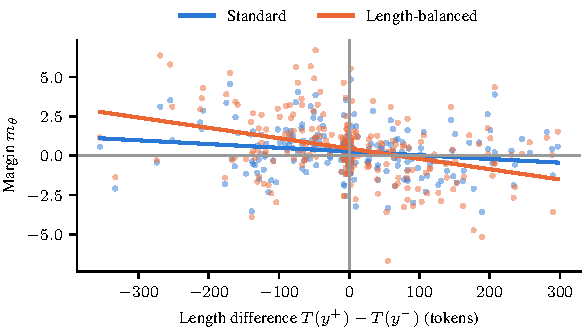
\includegraphics{figures/t1_length.pdf}
  \caption{DPO margin against the preferred-minus-rejected length difference on the 246 stratified pairs, with least-squares lines. The margin falls as the preferred response gets longer.}
  \label{fig:dpo-length}
\end{figure}

% let Figure 3 float past this heading so page 11 fills
{\renewcommand{\FloatBarrier}{}\section{Proximal Policy Optimization: Supplementary Results}}
\label{app:ppo}

\paragraph{Standard continuation.} Figure~\ref{fig:ppo-traj} shows the per-update quantities of the standard 20-update run. Each update drew a new prompt, so reward (panel a) and length (panel h) moved together from update to update. The clip fraction stayed at 0 in every update (panel f), while the pre-clip gradient norm passed the threshold of 1.0 in 3 of 20 updates (panel g).

\begin{figure}[!htb]
  \centering
  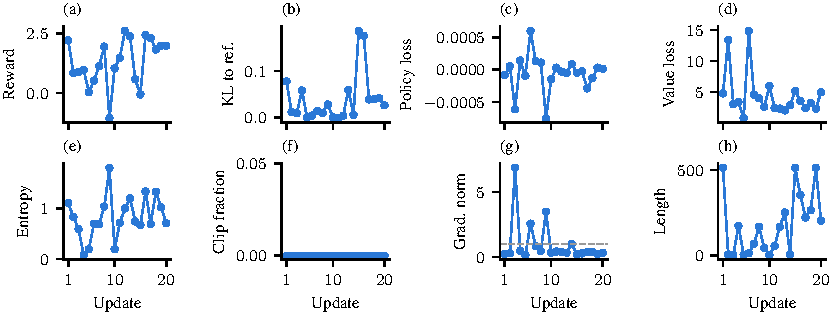
\includegraphics[width=\linewidth]{figures/x_ppo_traj.pdf}
  \caption{Standard PPO continuation with one new prompt per update. Panels show (a) reward minus the missing-EOS penalty, (b) KL, (c) policy loss, (d) value loss, (e) entropy, (f) clip fraction, (g) pre-clip gradient norm with the threshold dashed, and (h) length. The ratio clip never engaged, while the gradient clip acted in 3 of 20 updates.}
  \label{fig:ppo-traj}
\end{figure}

\paragraph{Clipping.} Table~\ref{tab:ppo-clip} reports the clip and affected fractions on the 32 cached rollouts after one epoch. The common field replays every $\epsilon$ on the $\epsilon = 0.20$ trajectory, and the own field lets each $\epsilon$ follow its own updates. Only $\epsilon = 0.05$ on its own trajectory clipped any token (0.0001), and no clipped token lost its gradient.

\begin{table}[!htb]
  \centering
  \caption{Clipping on the 32 cached rollouts after one epoch, on the common ($\epsilon = 0.20$) and each $\epsilon$'s own trajectory. Almost no ratio left even the narrowest band.}
  \label{tab:ppo-clip}
  \tablebody{tables/t2_clip.tex}
\end{table}

\paragraph{Compute.} Table~\ref{tab:compute} gives the peak GPU memory and wall-clock time of the standard PPO and GRPO runs. GRPO used more of both because it generated $K = 4$ completions per update against one response for PPO.

\begin{table}[!htb]
  \centering
  \caption{Peak GPU memory and wall-clock time of the standard 20-update PPO and GRPO runs on one L4 GPU. GRPO cost more because it samples four completions per update.}
  \label{tab:compute}
  \tablebody{tables/x_compute.tex}
\end{table}

\section{Group Relative Policy Optimization: Supplementary Results}
\label{app:grpo}

\paragraph{Standard continuation.} In Figure~\ref{fig:grpo-traj}, rings mark the three updates without a gradient. In updates 5 and 10 all four completions were identical (``HELLO WORLD'' for a Morse-code prompt and ``0'' for a date-validation prompt), so $\sigma_r = 0$ (panel b). In update 15 all four completions reached the 512-token cap and were masked, although their rewards ranged from $-1.14$ to 1.08. The four largest gradient norms (1.34 to 1.71, panel f) came from updates whose completions averaged 6 to 83 tokens (panel h), as expected from the $1/T_k$ weight.

\begin{figure}[!htb]
  \centering
  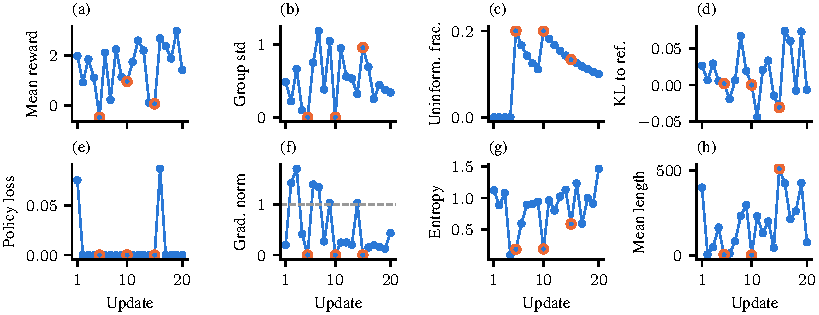
\includegraphics[width=\linewidth]{figures/x_grpo_traj.pdf}
  \caption{Standard GRPO continuation with $K = 4$ completions per update. Panels show (a) group mean reward, (b) within-group standard deviation, (c) uninformative-group fraction so far, (d) KL, (e) policy loss, (f) gradient norm with the threshold dashed, (g) entropy, and (h) mean length. Rings mark the three updates without a gradient.}
  \label{fig:grpo-traj}
\end{figure}

\section{Safety Calibration: Supplementary Results}
\label{app:safety}

\paragraph{Unsafe contrasts by category.} Figure~\ref{fig:safety-unsafe} shows, for each of the 8 unsafe contrast categories, the share of responses the judge did not label a justified refusal, all of which it labelled safe answers (Table~\ref{tab:safety-rates}). Only the discrimination contrasts stand out, at 10 to 14 of 25 per policy.

\begin{figure}[!htb]
  \centering
  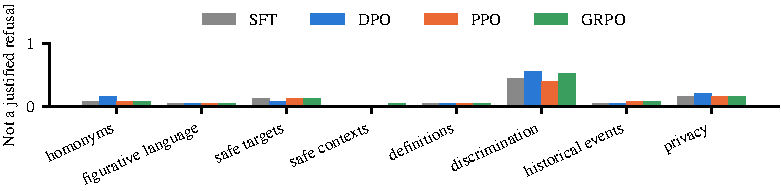
\includegraphics[width=\linewidth]{figures/t4_types_unsafe.pdf}
  \caption{Share of unsafe contrast prompts (25 per category) that the AI judge did not label a justified refusal (higher is worse), all of which it labelled safe answers. The judge failed mainly on discrimination contrasts.}
  \label{fig:safety-unsafe}
\end{figure}

\section{Feedback Source: Supplementary Results}
\label{app:feedback}

\paragraph{Verifier and judge agreement.} For each of the 300 GSM8K problems, both mechanisms compared the policy's response with SFT's. Table~\ref{tab:fb-agree} counts the problems where the verifier preferred one response and the judge picked the same one, and the problems the verifier tied where the judge picked a side.

\begin{table}[H]
  \centering
  \caption{Verifier and AI judge on the 300 GSM8K comparisons of each policy against SFT. The judge rarely agreed with the verifier when it was decisive and rarely broke its ties.}
  \label{tab:fb-agree}
  \tablebody{tables/x_agreement.tex}
\end{table}

\end{document}
